\documentclass{article}[12 pt,a4paper]
\usepackage[margin=2.5cm ,a4paper]{geometry}
\usepackage{amsmath}

\setlength{\parskip}{1ex} %--skip lines between paragraphs
\setlength{\parindent}{0pt} %--don't indent paragraphs

\linespread{1.25}

\usepackage{graphicx, caption, subcaption, float, hyperref}
%\usepackage[paper=a4paper,margin=25mm               % 25mm margins
    %        ]{geometry}

\usepackage[toc,page]{appendix}
\usepackage{tikz}
\usetikzlibrary{chains}
\usepackage[outdir=./]{epstopdf}

\title{Vulnerability Assessment Report  for\\
NightLider Pte Ltd}
\date{Chong Yun Long / Consultant @{\emph{Pwned Consulting}}}
% \date{\emph{\emph{Pwned Consulting}}}
\begin{document}

\maketitle
\newpage 
\tableofcontents
\newpage 



%Task 1:
%     1. Smashed stack layout explanation: 10 marks
%     2. Finding the correct addresses: 20 marks
%     3. Getting the shell: 10 marks
%     
%Task 2:
%     1. Explanation of address randomization: 10 marks
%     2. Explain why they can prevent the exploit, using information you get from GDB: 10 marks
% 
%Task 3:
%     1. Explanation of the mechanism of StackGuard protector: 10 marks
%     2. Explain why they can prevent the exploit, using information you get from GDB: 10 marks
% 
%Task 4: 
%     1. Explanation of the non-executable stack mechanism: 10 marks
%     2. Explain why they can prevent the exploit, using information you get from GDB: 10 marks


\section{Security Assessment Agreement}

\emph{Lider Corp} has authorized \emph{Pwned Consulting} to carry out a Vulnerability Assessment of its internal network systems.
An agreement between both parties has been arranged where the purpose is the discovery of security vulnerabilities in its network systems. 

\subsection{Fees \& Timing}
All testing and assessment work will be performed solely on Client's company premises, Monday -- Friday, 8 a.m. -- 8 p.m. local time. Work required outside of these normal business hours will incur an upcharge, to be approved by customer in advance. Automated testing may be performed outside of this window if testing can be scheduled in advance.

Any additional work required beyond our current estimate will be added to our invoices at the agreed daily billing rate.

\subsection{Disclaimer}

\emph{Pwned Consulting} and the Client have agreed to the following terms and conditions with regards to the vulnerability assessment services provided by \emph{Pwned Consulting}.

\begin{enumerate}
\item Client understands that \emph{Pwned Consulting} may use various methods and software tools to probe network resources for security-related information and to detect actual or potential security flaws and vulnerabilities. 
\item Client authorises \emph{Pwned Consulting} to perform such Security Services (and all such tasks and tests reasonably contemplated by or reasonably necessary to perform the Security Services or otherwise approved by Client from time to time) on network resources with the IP Addresses identified by Client
\item Client represents that, if Client does not own such network resources, it will have obtained consent and authorisation from the applicable third party, in form and substance satisfactory to \emph{Pwned Consulting}, to permit \emph{Pwned Consulting} to provide the Security Services. 
\item The services offered, such as penetration testing or vulnerability assessments, may also entail buffer overflows, fat pings, operating system specific exploits, and attacks specific to custom coded applications but will exclude intentional and deliberate Denial of Service Attacks.
\item Client acknowledges that the Security Services described herein could possibly result in service interruptions or degradation regarding the Client's systems and accepts those risks and consequences.
\item Client hereby consents and authorises Consultant to provide any or all the Security Services with respect to the Client's systems.
\item Client acknowledges it is the Client's responsibility to restore network computer systems to a secure configuration after Consultant testing. 
\end{enumerate}

\section{Methodology}

\subsection{Tools used}
As part of this security assessment, we have made use of the following tools:

\begin{description}
\item[\href{https://nmap.org/}{Nmap}] -- a free and open source utility for network discovery and security auditing. It can be used for network inventory, managing service upgrade schedules, and monitoring host or service uptime.
\item[\href{https://nmap.org/zenmap/}{Zenmap}] -- Zenmap is the official Nmap Security Scanner GUI
\item[\href{https://www.tenable.com/products/nessus-vulnerability-scanner}{Nessus Vulnerability Scanner}] --  Vulnerability scanner is developed by Tenable Network Security\footnote{http://www.tenable.com/}. It is able to scan for:
\begin{enumerate}
\item Vulnerabilities on a computer system
\item System misconfiguration
\item Default passwords
\item Denials of service using malformed packets
\item PCI DSS audits
\end{enumerate}
\end{description}

\subsection{Approach}

The security assessment will consist of two components, Reconnaissance and Vulnerability Scanning. 
\begin{enumerate}
\item Reconnaissance -- Zenmap/Nmap will be used to visualize network topology as well as to fingerprint the systems that are on the network. 
\item Vulnerability Scan --Nessus scanner will be used to identify and rank vulnerabilities of a target machine. Remediation measures/solutions will then be proposed to help better secure the system.
\end{enumerate}

\section{Reconnaissance}

\subsection{Topology}

\emph{Lider Corp} has provided us their network topology, as shown in Figure~\ref{network_diag}. They have requested that we focus our effort on \texttt{192.168.134.131}, a machine which has been targeted for attacks multiple times.

\begin{figure}
\centering
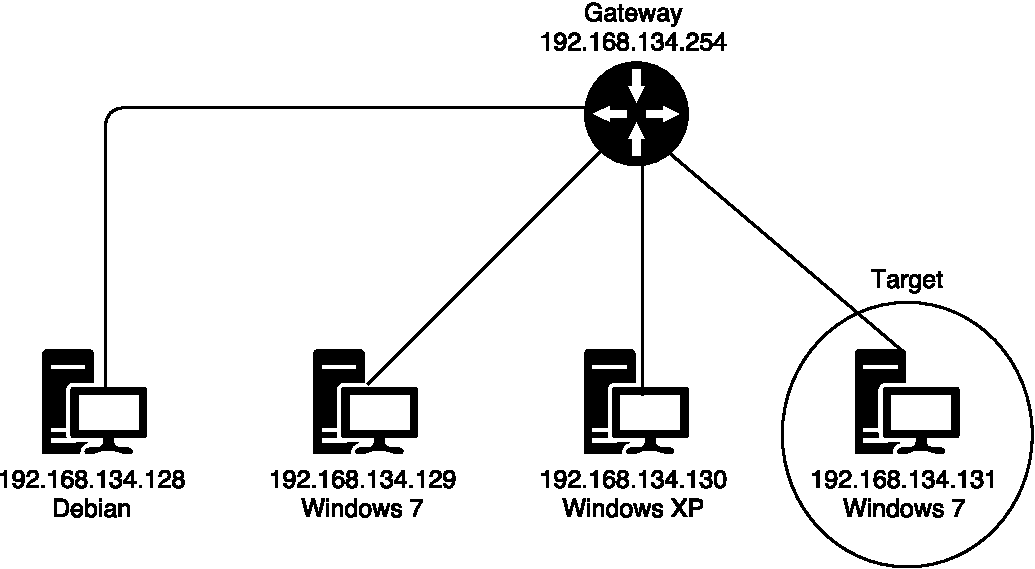
\includegraphics[width=0.6\textwidth]{scan/network_diag}
\caption{\emph{Lider Corp}'s network topology}
\label{network_diag}
\end{figure}

\subsection{Network Scan}
 
We conduct a network scan by running \texttt{nmap -T4 -A -v 192.168.134.128/24} in Zenmap, as shown in Figure~\ref{nmap_command}. The flags used were:
\begin{description}
\item[T4] Equivalent to --max-rtt-timeout 1250ms --min-rtt-timeout 100ms --initial-rtt-timeout 500ms --max-retries 6 and sets the maximum TCP scan delay to 10 milliseconds
\item[A] Enable OS detection, version detection, script scanning, and traceroute
\item[v] Verbose output
\end{description}

\begin{figure}
\centering
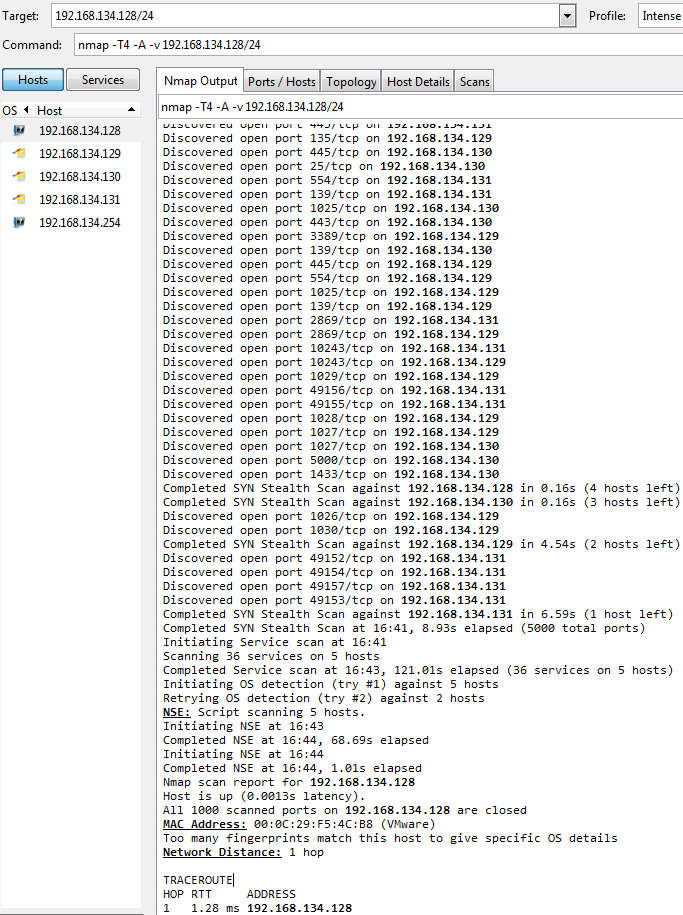
\includegraphics[width=0.7\textwidth]{scan/nmap_6}
\caption{Zenmap/Nmap interface and command used}
\label{nmap_command}
\end{figure}


The results of our scan revealed a network topology (Figure~\ref{nmap_topo}) that is similar to what was described to us by \emph{Lider Corp}. We also know that the target (\texttt{192.168.134.131}) is likely Windows 7 machine from the Nmap results (Figure~\ref{nmap_fingerprint})

\begin{figure}
        \centering
        \begin{subfigure}{0.4\textwidth}
		\centering
		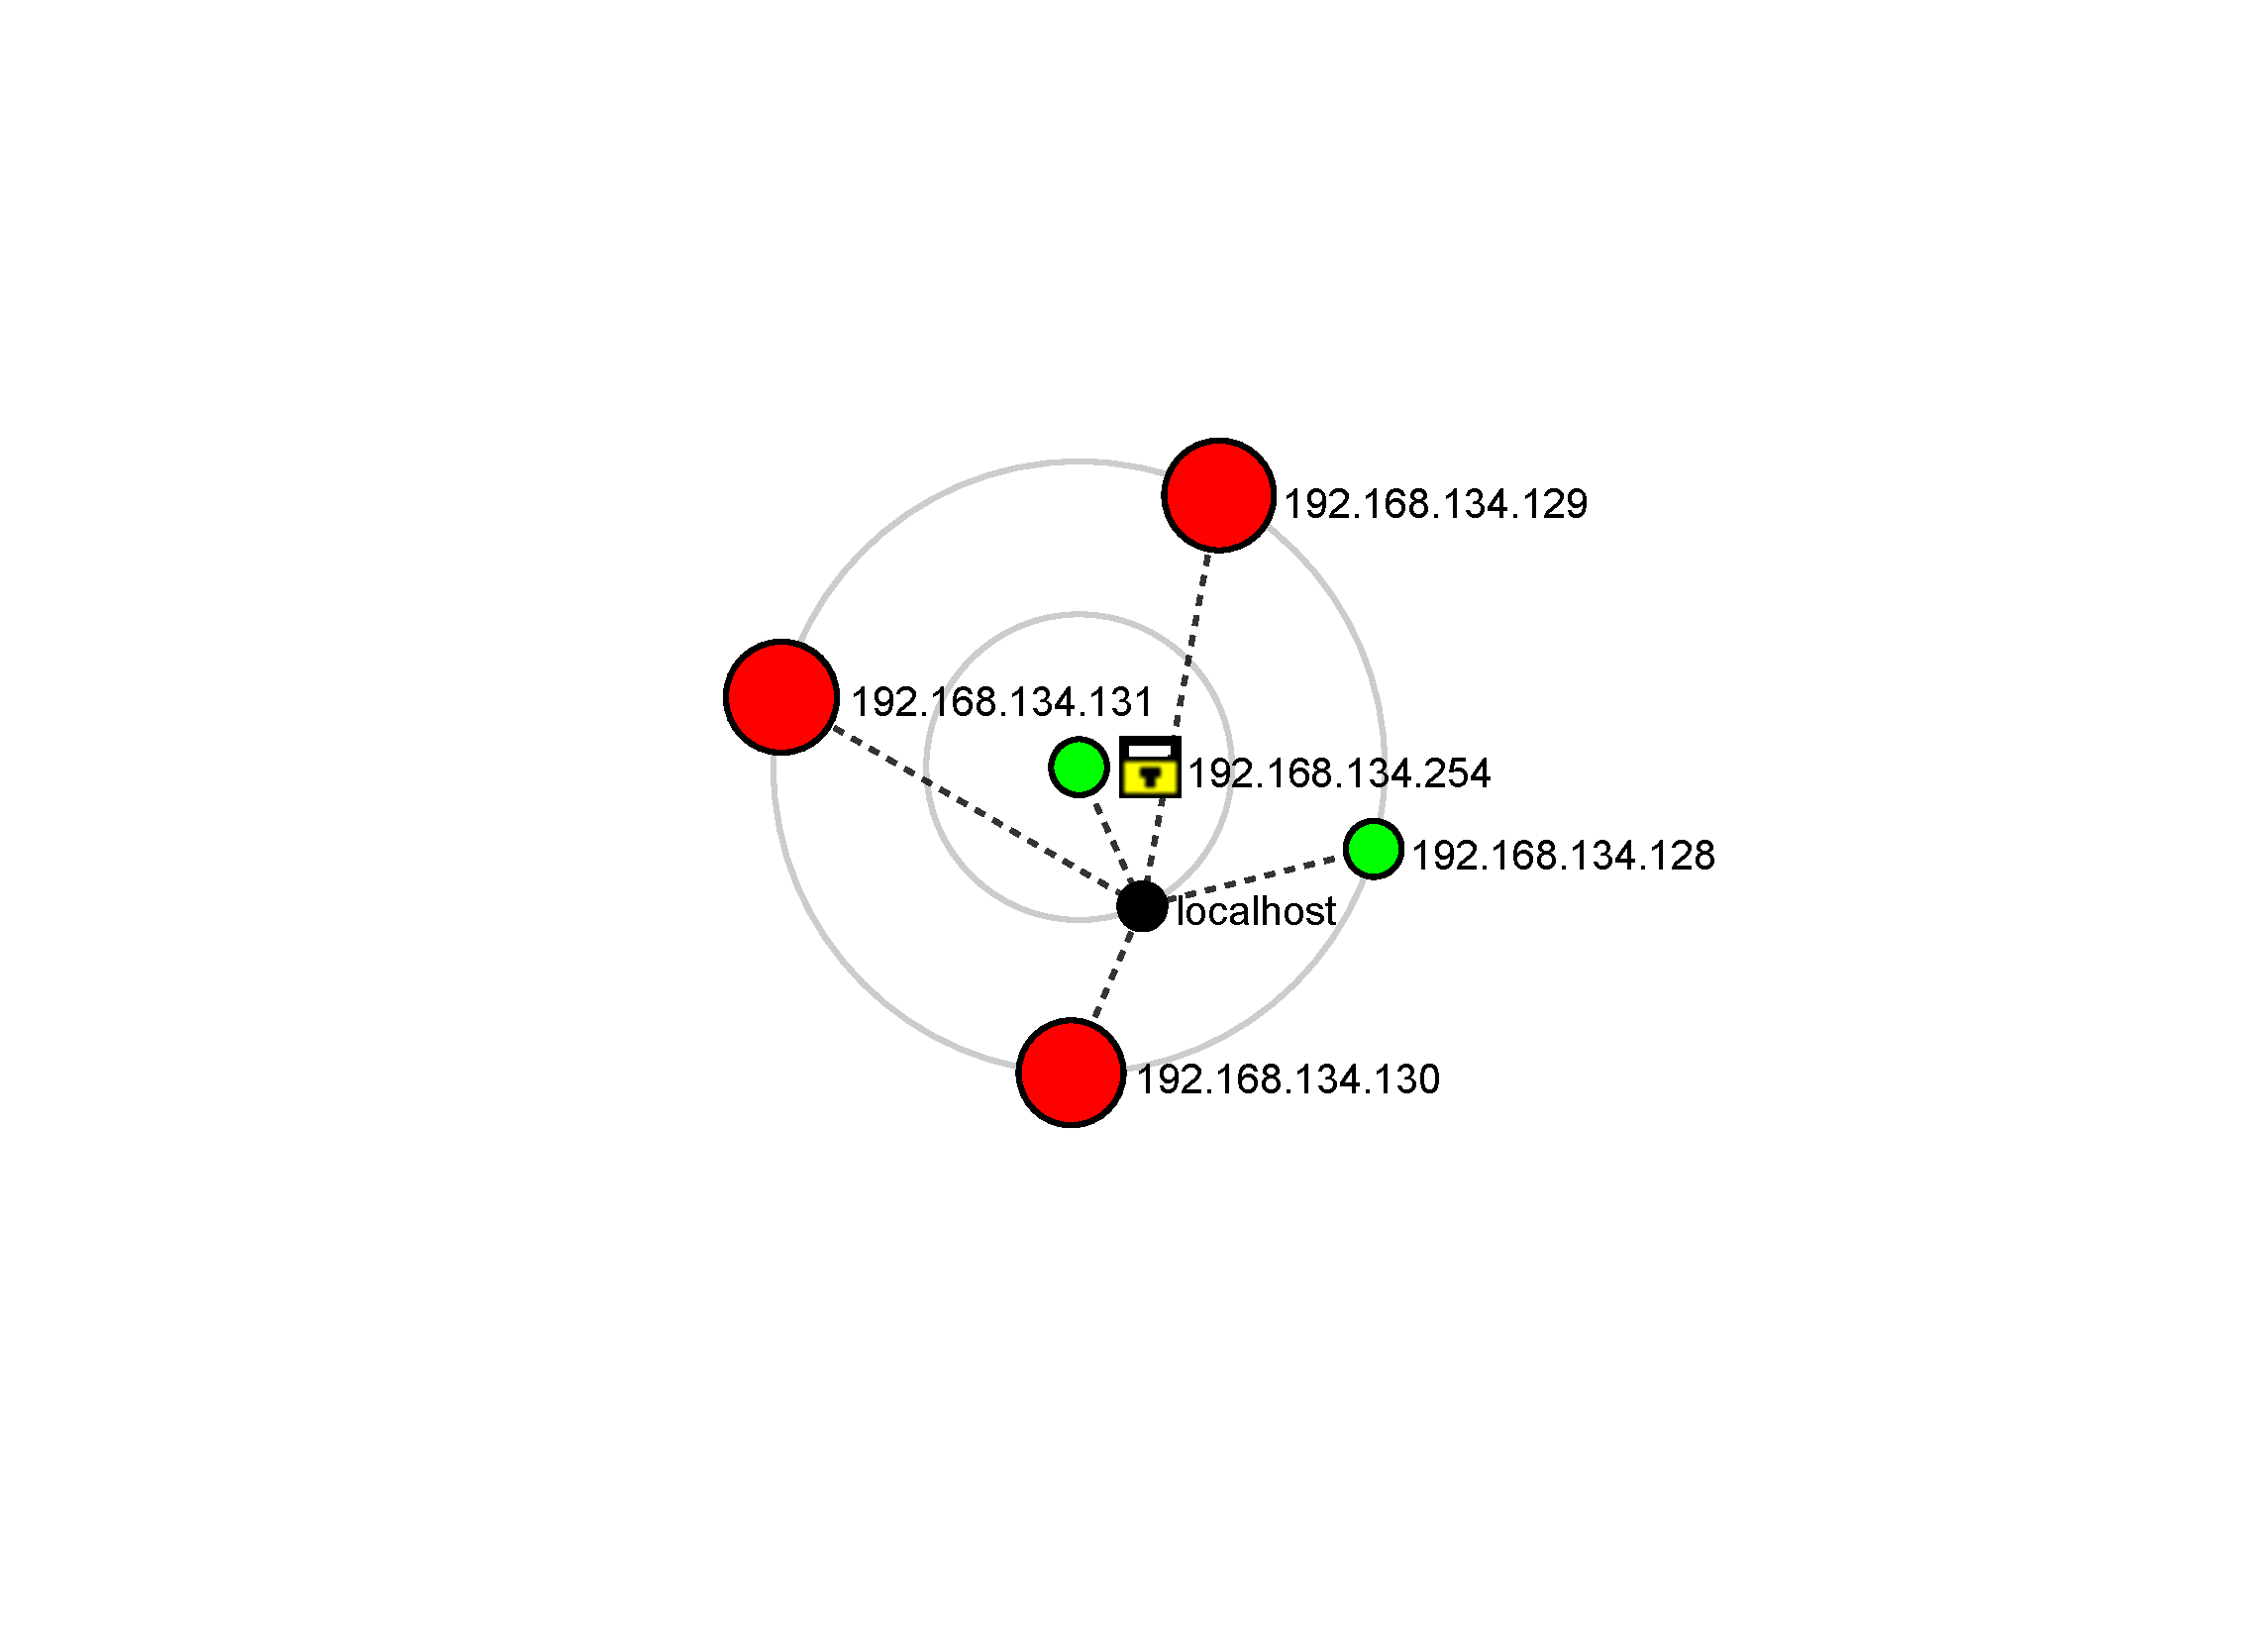
\includegraphics[width=0.7\textwidth]{scan/nmap_topo}
		\caption{\emph{Network topology from Nmap scan}}
		\label{nmap_topo}
        \end{subfigure}%
        ~ %add desired spacing between images, e. g. ~, \quad, \qquad etc.
          %(or a blank line to force the subfigure onto a new line)
        \begin{subfigure}{0.6\textwidth}
                \centering
                \includegraphics[width=\textwidth, page=7]{scan/nmap_5_selected}
                \caption{OS fingerprinting}
                \label{nmap_fingerprint}
        \end{subfigure}
        \caption{Nmap results}
\end{figure}

\section{Vulnerability Scan}

With information about the network, the next step would be to make use of Nessus to scan our target for system vulnerabilities. Since the target machine is running Windows, we can decrease the scanning duration by disabling plugins which are not applicable for Windows. In Figure~\ref{nessus_plugin}, AIX local security checks and CISCO plugins were disabled. There are many other unrelated plugins that we are able to disable to speed up the scanning process.

\begin{figure}
\centering
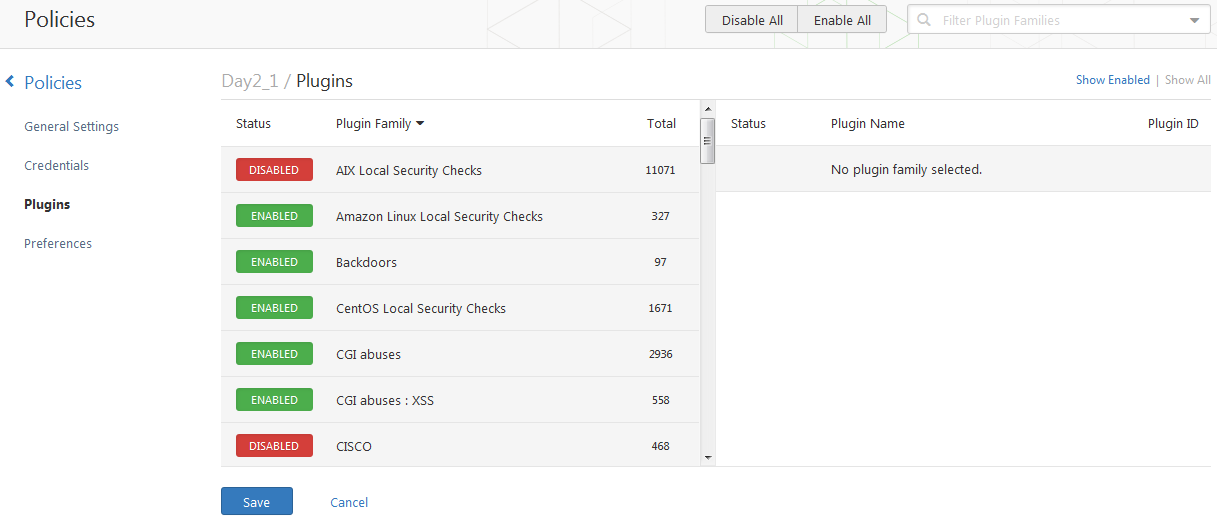
\includegraphics[width=1\textwidth]{scan/nessus_1}
\caption{Disabling unnecessary Nessus plugins}
\label{nessus_plugin}
\end{figure}

The Nessus scan on our target revealed 1 high, 6 medium and 2 low vulnerabilities (Figure~\ref{nessus_scan}). The detailed Nessus report (Figure~\ref{nessus_report}) revealed that the vulnerability lies in the implementation of Remote Desktop Protocol (RDP) on the Windows host (MS12-020). Attackers are able to send crafted RDP packets to the host and execute code remotely
\begin{figure}
\centering
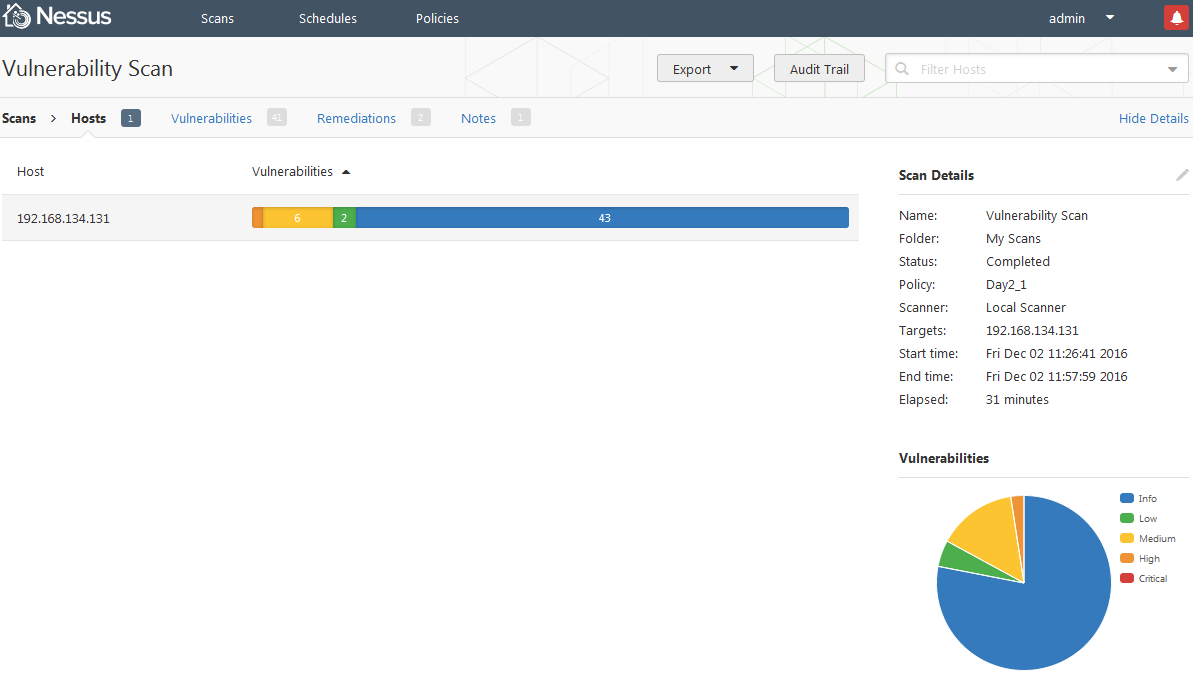
\includegraphics[width=1\textwidth]{scan/nessus_3}
\caption{Nessus scan results}
\label{nessus_scan}
\end{figure}


\begin{figure}
\centering
\includegraphics[width=0.8\textwidth, page=3]{scan/nessus_report}
\caption{Nessus indepth report}
\label{nessus_report}
\end{figure}

 
\subsection{Remediation}

Microsoft has released a patch on its security bulletin(MS12-020) site\footnote{\url{https://technet.microsoft.com/en-us/library/security/ms12-020.aspx}}. 

This security update resolves two privately reported vulnerabilities in the Remote Desktop Protocol. The more severe of these vulnerabilities could allow remote code execution if an attacker sends a sequence of specially crafted RDP packets to an affected system. By default, the Remote Desktop Protocol (RDP) is not enabled on any Windows operating system. Systems that do not have RDP enabled are not at risk.
This security update is rated Critical for all supported releases of Microsoft Windows. For more information, see the subsection, Affected and Non-Affected Software, in this section.
The security update addresses the vulnerabilities by modifying the way that the Remote Desktop Protocol processes packets in memory and the way that the RDP service processes packets. For more information about the vulnerabilities, see the Frequently Asked Questions (FAQ) subsection for the specific vulnerability entry under the next section, Vulnerability Information.
Recommendation. The majority of customers have automatic updating enabled and will not need to take any action because this security update will be downloaded and installed automatically. Customers who have not enabled automatic updating need to check for updates and install this update manually. For information about specific configuration options in automatic updating, see Microsoft Knowledge Base Article 294871.
For administrators and enterprise installations, or end users who want to install this security update manually, Microsoft recommends that customers apply the update immediately using update management software, or by checking for updates using the Microsoft Update service.
See also the section, Detection and Deployment Tools and Guidance, later in this bulletin.
Known Issues. Microsoft Knowledge Base Article 2671387 documents the currently known issues that customers may experience when installing this security update. The article also documents recommended solutions for these issues.
Affected and Non-Affected Software
The following software have been tested to determine which versions or editions are affected. Other versions or editions are either past their support life cycle or are not affected. To determine the support life cycle for your software version or edition, visit Microsoft Support Lifecycle.

We recommend LiderCorp to apply the patch immediately to the affected system. 

Remote Desktop is a huge attack surface for the Windows operating system. It is highly recommended to disable Remote Desktop on all Windows systems which do not require Remote Desktop functionalities. 

\end{document}
